% \documentclass[12pt, a4paper, oneside]{ctexart}
\documentclass[12pt, oneside]{ctexart}
\usepackage{amsmath, amsthm, amssymb, bm, color, enumerate, framed, graphicx, longtable, mathrsfs, subfigure, tikz}
% \usepackage[dvipsnames]{xcolor}
% \usepackage{geometry}
\usepackage[a4paper, total={145mm,210mm}]{geometry}
\geometry{left=2.54cm,right=2.54cm,top=3.18cm,bottom=3.18cm}
\usepackage{pdfpages}

%按章节编号
\numberwithin{figure}{section}
\numberwithin{table}{section}

% 超链接设置
\usepackage{hyperref}
\hypersetup{  
    colorlinks = true,    % 更改链接颜色  
    linkcolor = black,      % 链接颜色  
    urlcolor = blue,        % URL 颜色  
    citecolor = green,     % 引用颜色  
    % underline = true,  
    linkbordercolor = red,
}
% \hypersetup{colorlinks=true,linkcolor=black}


%代码包设置
\usepackage{listings}
\lstset{
    basicstyle          =   \sffamily,          % 基本代码风格
    keywordstyle        =   \bfseries,          % 关键字风格
    commentstyle        =   \rmfamily\itshape,  % 注释的风格,斜体
    stringstyle         =   \ttfamily,  % 字符串风格
    flexiblecolumns,                % 别问为什么,加上这个
    numbers             =   left,   % 行号的位置在左边
    showspaces          =   false,  % 是否显示空格,显示了有点乱,所以不现实了
    numberstyle         =   \zihao{-5}\ttfamily,    % 行号的样式,小五号,tt等宽字体
    showstringspaces    =   false,
    captionpos          =   t,      % 这段代码的名字所呈现的位置,t指的是top上面
    frame               =   lrtb,   % 显示边框
}
\lstdefinestyle{C}{
    language        =   C, % 语言选C
    basicstyle      =   \zihao{-5}\ttfamily,
    numberstyle     =   \zihao{-5}\ttfamily,
    keywordstyle    =   \color{blue},
    keywordstyle    =   [2] \color{teal},
    stringstyle     =   \color{magenta},
    commentstyle    =   \color{red}\ttfamily,
    breaklines      =   true,   % 自动换行,建议不要写太长的行
    columns         =   fixed,  % 如果不加这一句,字间距就不固定,很丑,必须加
    basewidth       =   0.5em,
}



% 设置思源宋体为中文字体
\setCJKsansfont{Source Han Serif SC}

% 设置思源黑体为中文字体
\setCJKsansfont{Source Han Sans SC}

% 设置arev为英文字体
\setsansfont{Arev Sans}

% 字体颜色
\def\red{\color{red}}
\def\blue{\color{blue}}
\def\black{\color{black}}
\def\green{\color{green}}

\CTEXsetup[format={\Large\bfseries}]{section}

\definecolor{shadecolor}{RGB}{241, 241, 255}
\newcounter{problemname}
\newenvironment{problem}{\begin{shaded}\stepcounter{problemname}\par\noindent\textbf{题目\arabic{problemname}. }}{\end{shaded}\par}
\newenvironment{solution}{\par\noindent\textbf{解答. }}{\par}
\newenvironment{note}{\par\noindent\textbf{题目\arabic{problemname}的注记. }}{\par}
%\renewcommand{\proofname}{\bf 证明}

\begin{document}

\thispagestyle{empty}

\begin{figure}[t]
    \centering
    
\includegraphics[width=13cm]{images/logo.png}
\end{figure}

\vspace*{\fill}
    \begin{center}
        \Huge\textbf{数据库原理}
    \end{center}
    \rightline{\LARGE\textbf{——课程作业}}
\vspace*{\fill}

\begin{table}[b]
    \centering
    \large
    \begin{tabular}{ll}
    \textbf{课程:} & 数据库原理 \\
    \textbf{班级:} & 1621402 \\
    \textbf{姓名:} & 黄钰轩 \\
    \textbf{学号:} & 162140222 \\
    \textbf{教师:} & 郑吉平 \\
    \textbf{学期:} & 2023-2024 春季 \\
    \end{tabular}
\end{table}

\newpage
\pagenumbering{Roman}
\setcounter{page}{1}
\tableofcontents
\newpage
\setcounter{page}{1}
\pagenumbering{arabic}

\section{第一章作业}

\begin{problem}
    试述数据、数据库、数据库管理系统、数据库系统的概念.
\end{problem}

\begin{solution}
    \begin{enumerate}[(1)]
        \item 数据: 描述事物的符号记录.
        \begin{itemize}
            \item 在现实生活,数据是可识别的抽象符号,即描述事物的符号记录.
            \item 在计算机中,数据是所有能被计算机处理的符号的总称.
            \item 在数据库中,数据是数据库中存储的基本对象.
        \end{itemize}
        \item 数据库: 
        \begin{itemize}
            \item 一组相互有关联的数据集合.
            \item 长期储存在计算机中的有组织的、可管理和可共享的数据集合.
        \end{itemize}
        \item 数据库管理系统:
        \begin{itemize}
            \item 位于用户(应用程序)与操作系统之间的数据库管理软件.
            \item 一个管理数据的大型复杂基础软件系统.
        \end{itemize}
        \item 数据库系统: 
        \begin{itemize}
            \item 由数据库管理系统和相关工具组成的软件系统,用于管理和操作大量数据.
        \end{itemize}
    \end{enumerate}
\end{solution}

\begin{problem}
    试述数据模型的概念、作用及其包含的三个要素.
\end{problem}

\begin{solution}
    \begin{enumerate}[(1)]
        \item 数据库模型的概念:
        \begin{itemize}
            \item 数据模型是数据库结构的基础,它是描述数据(数据结构)、数据之间的联系,数据语义即数据操作,以及一致性(完整性)约束的\textbf{概念和工具的集合}.
        \end{itemize}
        \item 数据库模型的作用:
        \begin{itemize}
            \item 在数据库领域,数据模型被广泛用于表示这些数据库设计的“描述”,更好的刻画数据.
            \item 数据模型精确描述了系统的静态特性、动态特性和完整性约束条件.
        \end{itemize}
        \item 数据库模型的三个要素:
        \begin{itemize}
            \item 数据结构: 数据结构描述数据库的组成对象以及对象之间的联系.
            \item 数据操纵: 是指对数据库中各种对象(型)的实例(值)允许进行的操作的集合,包括操作及有关的操作规则,是对系统动态特性的描述.
            \item 完整性约束: 是一组完整性规则的集合. 完整性规则是给定的数据模型中数据及其联系所具有的制约和依存规则,用以限定符合数据模型的数据库状态以及状态的变化,以保证数据的正确、有效、相容.
        \end{itemize}
    \end{enumerate}
\end{solution}

\begin{problem}
    试述数据库系统的三级模式结构,并说明这种结构的优点是什么.
\end{problem}

\begin{solution}
    \begin{enumerate}[(1)]
        \item 数据库系统的三级模式结构由模式、外模式和内模式组成.
        \begin{itemize}
            \item 模式也称逻辑模式,是数据库中全体数据的逻辑结构和特征的描述,是所有用户的公共数据视图. 模式的一个具体值称为模式的一个实例.
            \item 外模式,亦称子模式或用户模式,是数据库用户(包括应用程序员和最终用户)能够看见和使用的局部数据的逻辑结构和特征的描述,是数据库用户的数据视图,是与某一应用有关的数据的逻辑表示.
            \item 内模式也称物理模式或存储模式,它是对数据物理结构和存方式的描述,是数据在数据库内部的组织方式.
        \end{itemize}
        \item 三级模式结构的优点:
        \begin{itemize}
            \item 数据库系统的三级模式是对数据的三个抽象级别,它把数据的具体组织留给数据库管理系统,使用户能逻辑抽象地处理数据,而不必关心数据在计算机中的具体表示方式和存储方式.
            \item 数据库系统在这三级模式之间提供了两层映像: 外模式/模式映像和模式/内模式映像. 正是这两层映像保证了数据库系统中的数据能够具有较高的逻辑独立性和物理独立性.
        \end{itemize}
    \end{enumerate}
\end{solution}

\begin{problem}
    试述数据与程序的物理独立性和逻辑独立性. 为什么数据库系统具有较强的数据与程序的独立性?
\end{problem}

\begin{solution}
    \begin{enumerate}[(1)]
        \item 
        \begin{itemize}
            \item 数据与程序的物理独立性: 当数据库的存储结构改变时(如选用了另一种存储结构),由数据库管理员对模式/内模式映像做相应改变,可以使模式保持不变,从而应用程序也不必改变,保证了数据与程序的物理独立性,简称数据的物理独立性.
            \item 数据与程序的逻辑独立性: 当模式改变时(例如增加新的关系、新的属性、改变属性的数据类型等),由数据库管理员对各个外模式/模式的映像做相应改变,可以使外模式保持不变. 应用程序是依据数据的外模式编写的,从而应用程序不必修改,保证了数据与程序的逻辑独立性,简称数据的逻辑独立性.
        \end{itemize}
        \item 数据库管理系统在三级模式之间提供的两层映像保证了数据库系统中的数据能够具有较高的逻辑独立性和物理独立性.
    \end{enumerate}
\end{solution}

\newpage
\section{第二章作业}
% 计数器置零
\setcounter{problemname}{0}

\begin{problem}
    试述关系模型的三个组成部分.
\end{problem}

\begin{solution}
    关系模型由关系数据结构、关系操作集合和关系完整性约束三部分组成.
    \begin{figure}[!htpb]
        \centering
        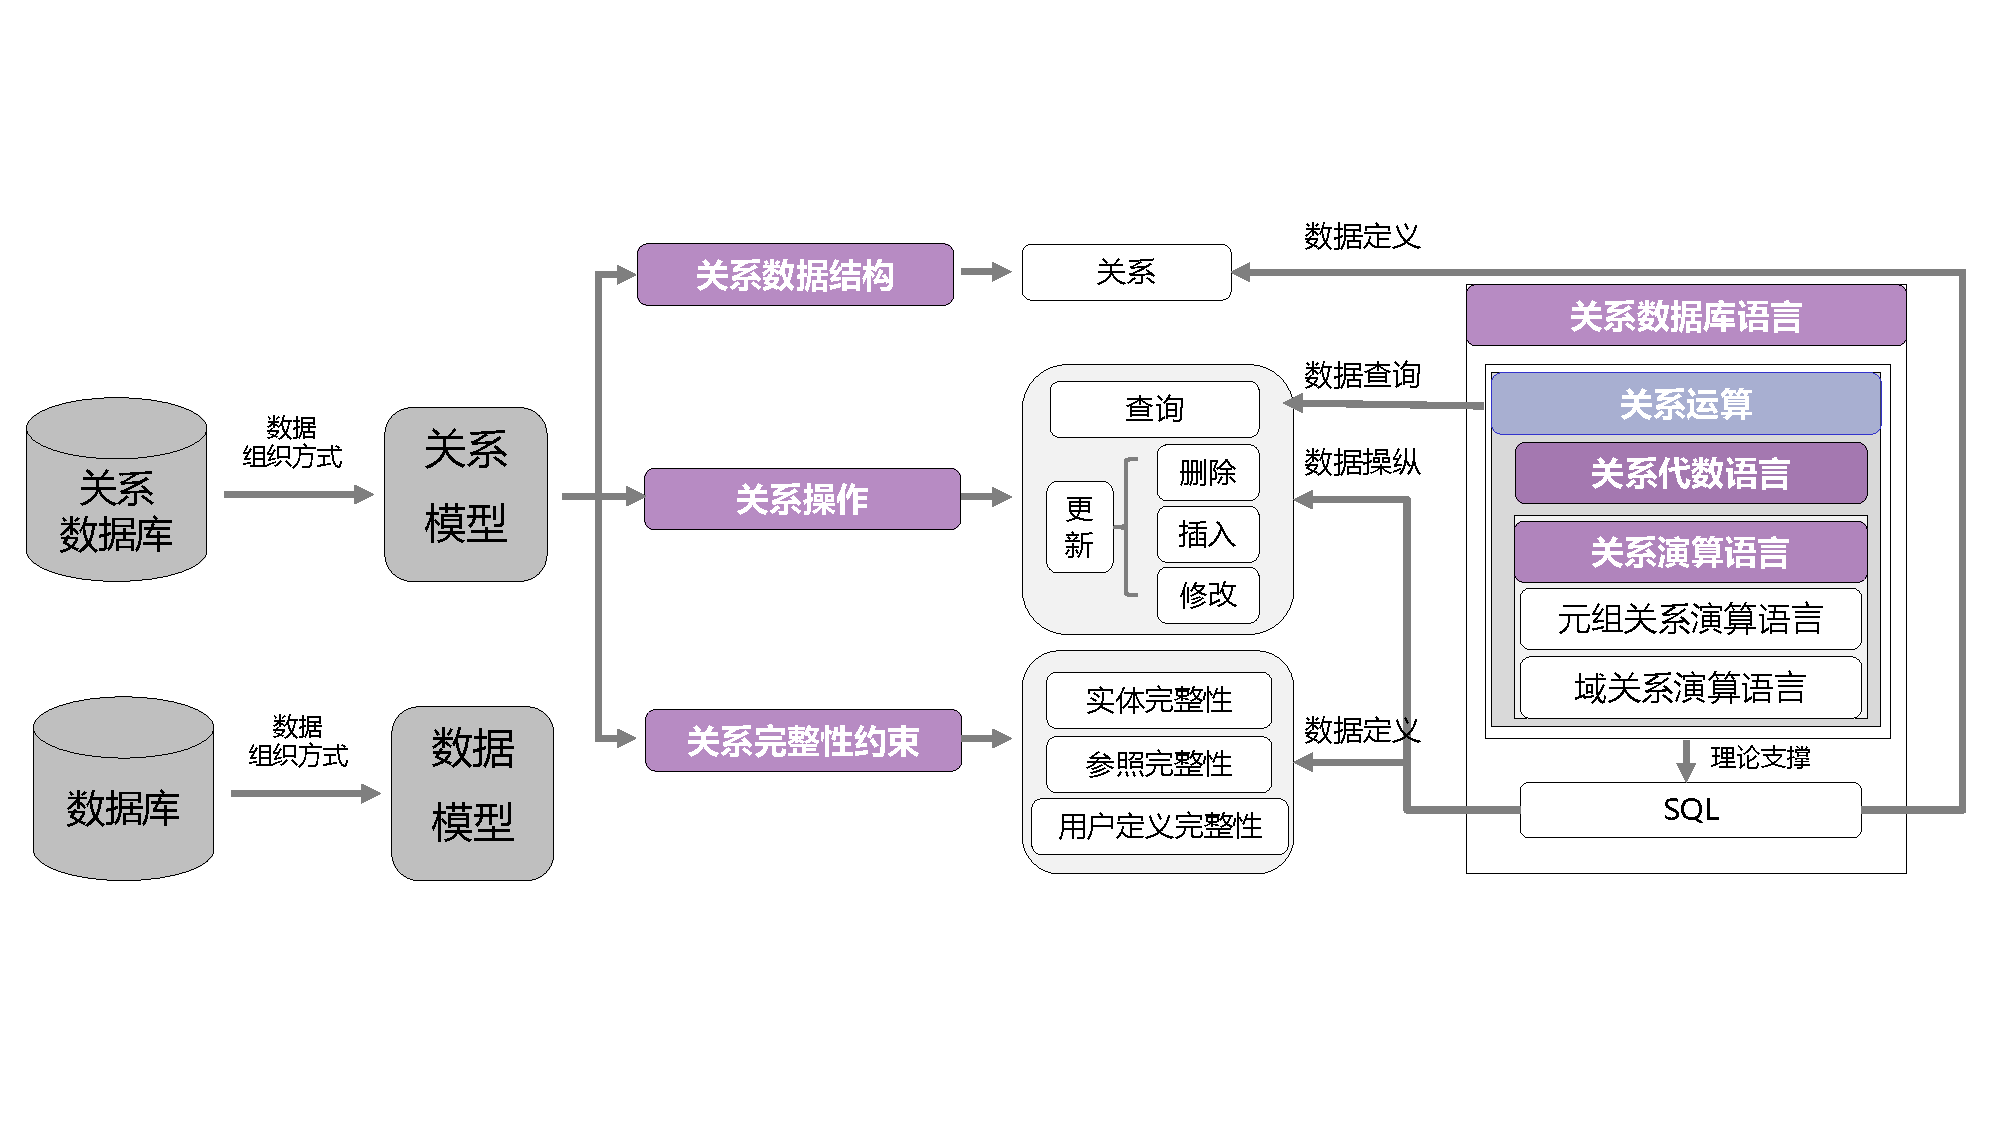
\includegraphics[width=15.5cm]{images/sec2/2-1_Relational_Model.pdf}
        \caption{关系模型框架}
        \label{fig2-1}
    \end{figure}
\end{solution}

\begin{problem}
    设有一个$\mathbf{SPJ}$数据库,包括四个关系模式 $\mathbf{S}$、$\mathbf{P}$、$\mathbf{J}$ 和$\mathbf{SPJ}$.
    $$\begin{aligned}
        & \mathrm{S(SNO, SNAME, STATUS, CITY);}  \\
        & \mathrm{P(PNO, PNAME, COLOR, WEIGHT);} \\
        & \mathrm{J(JNO, JNAME, CITY);}          \\
        & \mathrm{SPJ(SNO, PNO, JNO, QTY)};
    \end{aligned}$$

    供应商表$\mathbf{S}$由供应商代码(SNO)、供应商姓名(SNAME)、供应商状态(STATUS)、供应商所在城市(CITY)组成.

    零件表$\mathbf{P}$由零件代码(PNO)、零件名(PNAME)、颜色(COLOR)、重量(WEIGHT)组成.

    工程项目表$\mathbf{J}$由工程项目代码(JNO)、工程项目名(JNAME)、工程项目所在城市(CITY)组成.

    供应情况表$\mathbf{SPJ}$由供应商代码(SNO)、零件代码(PNO)、工程项目代码(JNO)、供应数量(QTY)组成,表示某供应商供应某种零件给某工程项目的数量为QTY.

    今有若干数据如 图 \ref{SPJ} 所示.

    试用关系代数、元组关系演算语言 ALPHA 完成如下查询:
    \begin{enumerate}[(1)]
        \item 求供应工程 J1 零件的供应商代码 SNO.
        \item 求供应工程 J1 零件 P1 的供应商代码 SNO.
        \item 求供应工程 J1 零件为红色的供应商代码 SNO.
        \item 求没有使用天津供应商生产的红色零件的工程号 JNO.
        \item 求至少使用了与供应商 S1 所供应的全部零件相同零件号的工程号 JNO.
    \end{enumerate}
\end{problem}

\begin{figure}[!htpb]
    \centering
    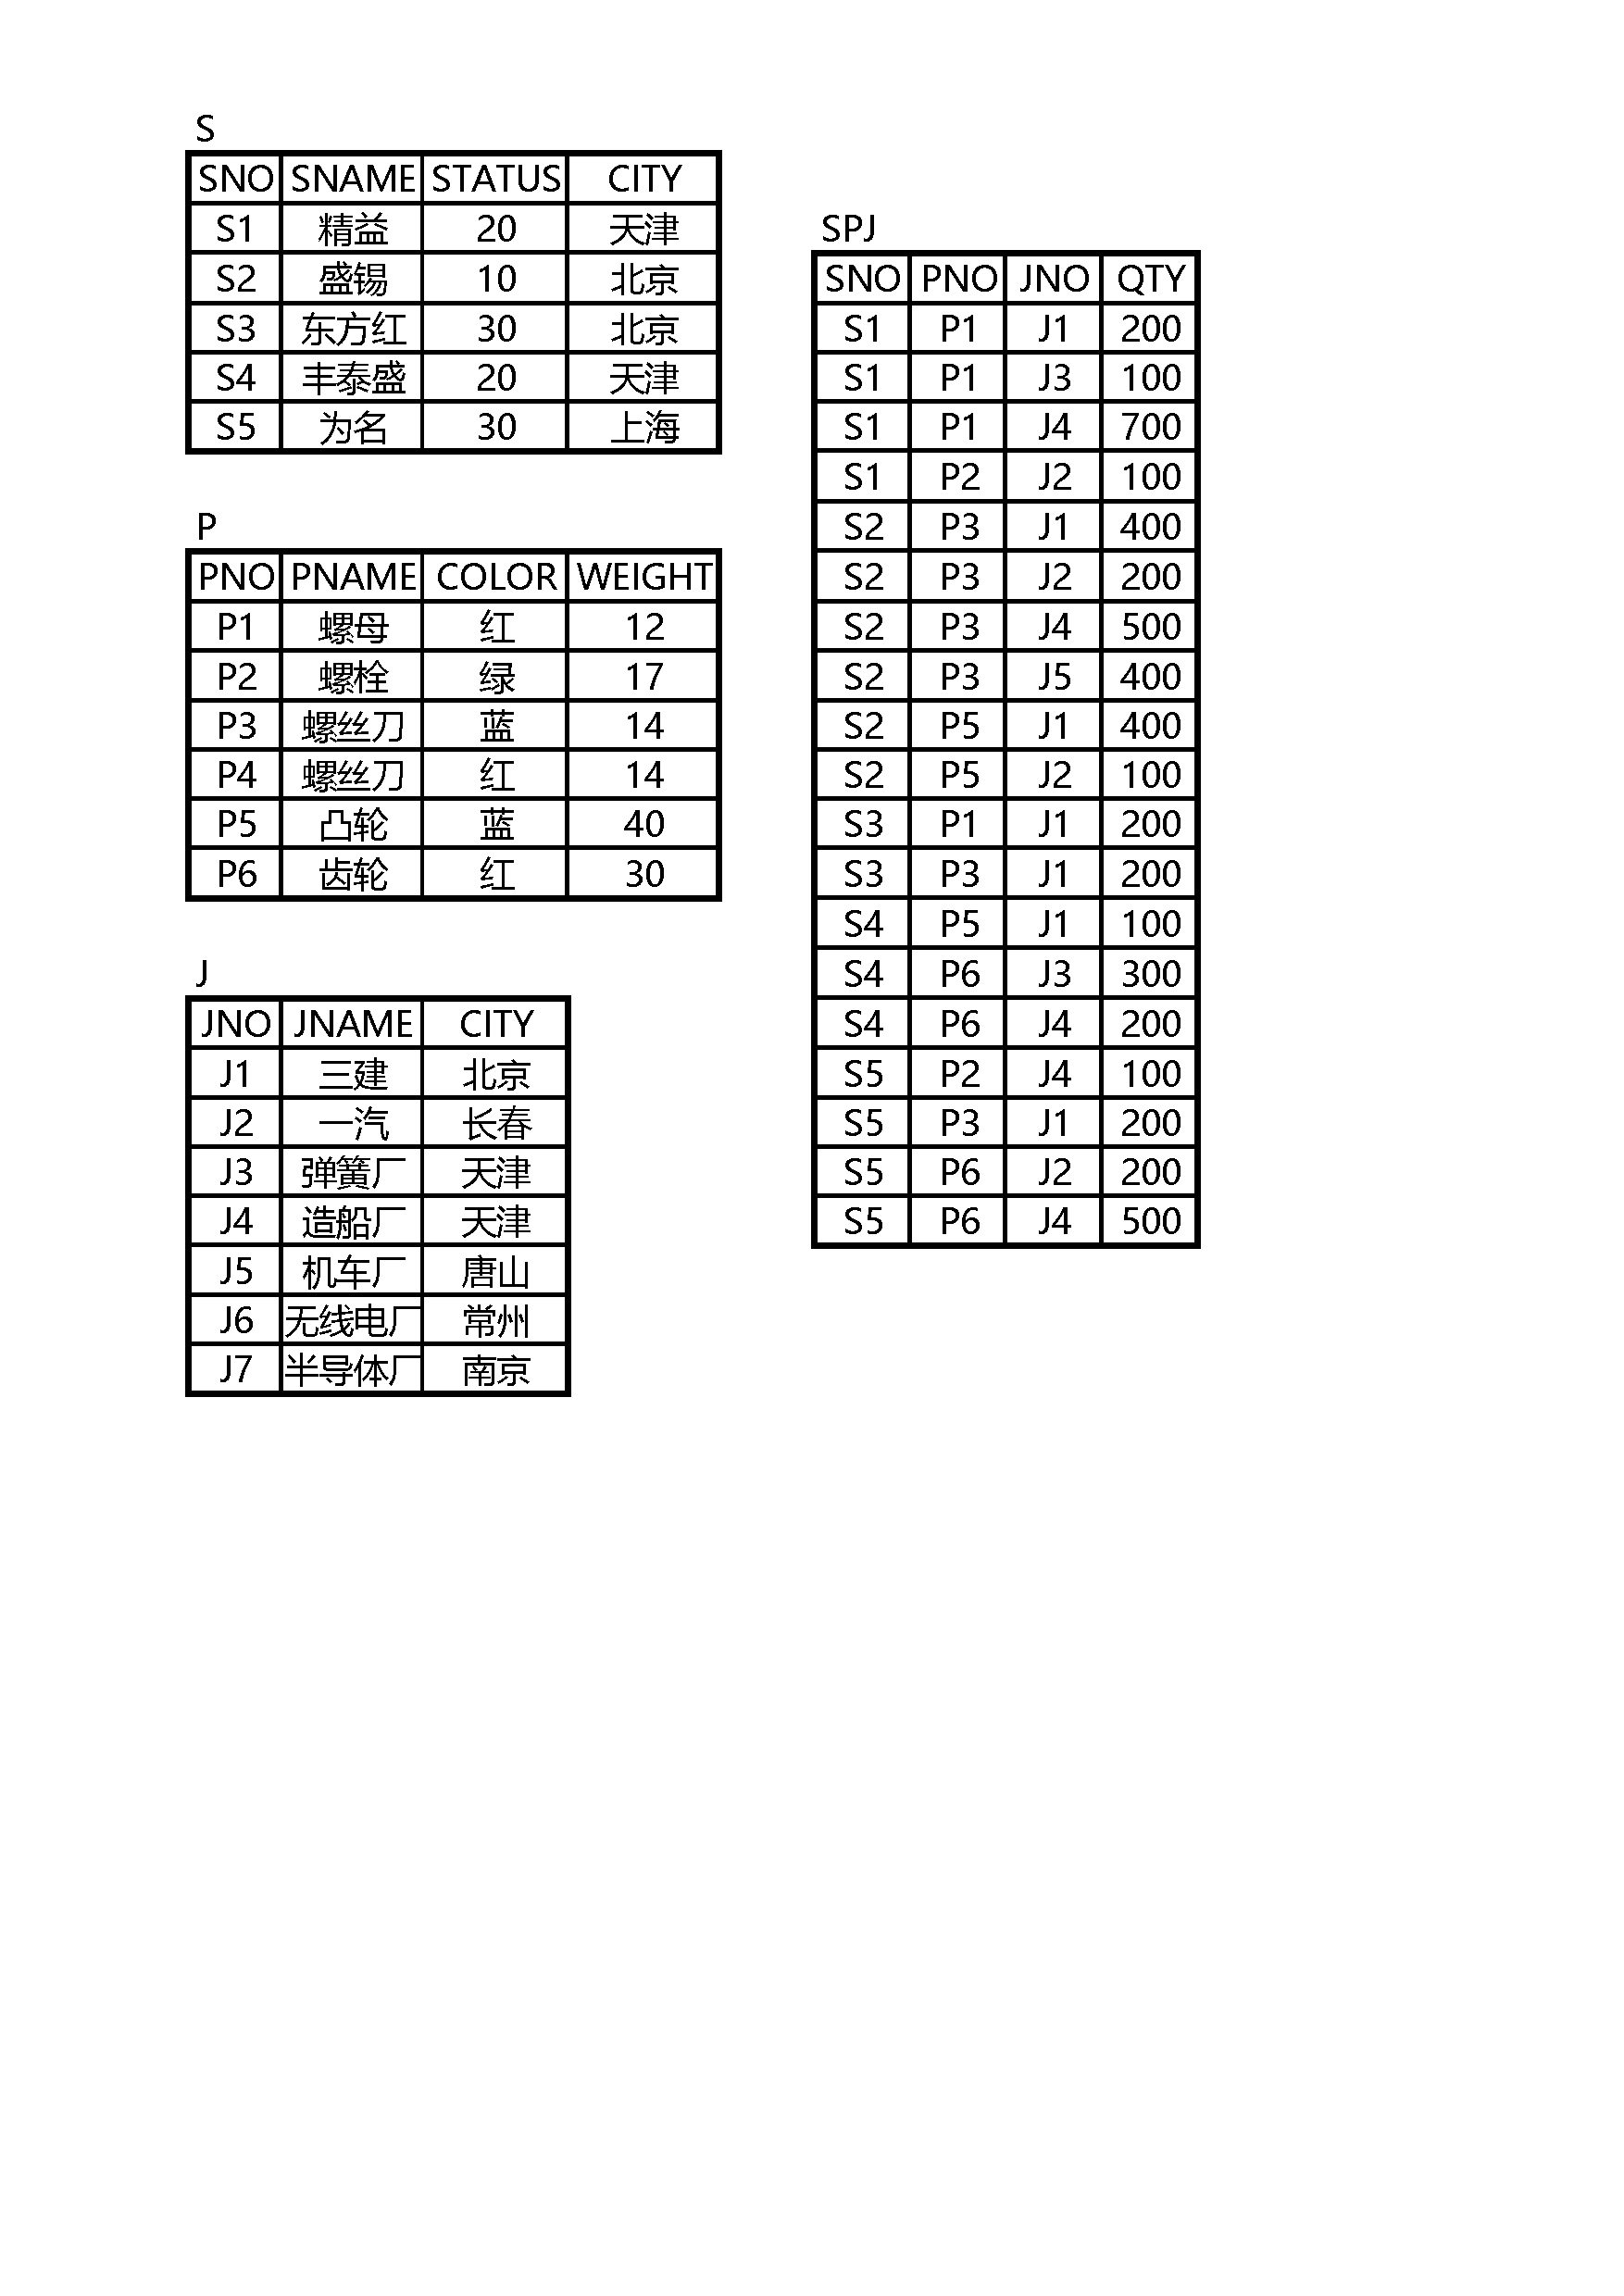
\includegraphics[width=13cm]{images/sec2/2-2_SPJ.pdf}
    \caption{SPJ 数据库数据}
    \label{SPJ}
\end{figure}

\begin{solution}
    \begin{enumerate}[(1)]
        \item
        \begin{itemize}
            \item 关系代数:
                  $$\Pi_{\mathrm{SNO}}(\sigma_{\mathrm{JNO} = '\mathrm{J1}'}(\mathbf{SPJ}))$$
            \item ALPHA语言:
                \lstinputlisting[
                    % style       =   C,
                    % caption     =   {\bf probe.c},
                    label       =   {3-1_code}
                ]{./code/sec2/3-1.txt}
        \end{itemize}
        \item
        \begin{itemize}
            \item 关系代数:
                  $$\Pi_{\mathrm{SNO}}(\sigma_{\mathrm{JNO} = '\mathrm{J1}' \land \mathrm{PNO} = '\mathrm{P1}'}(\mathbf{SPJ}))$$
            \item ALPHA语言:
                \lstinputlisting[
                    % style       =   C,
                    % caption     =   {\bf probe.c},
                    label       =   {3-2_code}
                ]{./code/sec2/3-2.txt}
        \end{itemize}
        \item
        \begin{itemize}
            \item 关系代数:
                  $$\Pi_{\mathrm{SNO}}(\Pi_{\mathrm{SNO}, \mathrm{PNO}}(\sigma_{\mathrm{JNO} = '\mathrm{J1}'}(\mathbf{SPJ})) \bowtie \Pi_{\mathrm{PNO}}(\sigma_{\mathrm{COLOR} = '\text{红}'}(\mathbf{P})))$$
            \item ALPHA语言:
                \lstinputlisting[
                        % style       =   C,
                        % caption     =   {\bf probe.c},
                        label       =   {3-3_code}
                    ]{./code/sec2/3-3.txt}
        \end{itemize}
        \item
        \begin{itemize}
            \item 关系代数:
            $$\Pi_{\mathrm{JNO}}(\mathbf{SPJ}) - \Pi_{\mathrm{JNO}}(\sigma_{\mathrm{CITY} = '\text{天津}' \land \mathrm{COLOR} = '\text{红}'}(\mathbf{S} \bowtie \mathbf{SPJ} \bowtie \mathbf{P}))$$
            \item ALPHA语言:
                \lstinputlisting[
                    % style       =   C,
                    % caption     =   {\bf probe.c},
                    label       =   {3-4_code}
                ]{./code/sec2/3-4.txt}
            \end{itemize}
        \item
        \begin{itemize}
            \item 关系代数:
                  $$\Pi_{\text{JNO},\text{PNO}}(\mathbf{SPJ}) \div \Pi_{\text{PNO}}(\sigma_{\text{SNO} = '\text{S1}'}(\mathbf{SPJ}))$$
            \item ALPHA语言:
                \lstinputlisting[
                    % style       =   C,
                    % caption     =   {\bf probe.c},
                    label       =   {3-5_code}
                ]{./code/sec2/3-5.txt}
        \end{itemize}
    \end{enumerate}
\end{solution}

\begin{problem}
    试述等值连接与自然连接的区别和联系.
\end{problem}

\begin{solution}
    \begin{itemize}
        \item 自然连接是一种特殊的等值连接.
        \item 自然连接将连接条件指定为$R$和$S$中属性名相同的列做等值连接,因此$p$可省略.
    \end{itemize}
\end{solution}
\newpage
\begin{note}
    以$\mathbf{Student}$、$\mathbf{SC}$表为例,
    $$\mathbf{Student}\bowtie_{\mathrm{Student.Sno = SC.Sno}}\mathbf{SC}$$
    结果如下:
    \begin{figure}[!htpb]
        \centering
        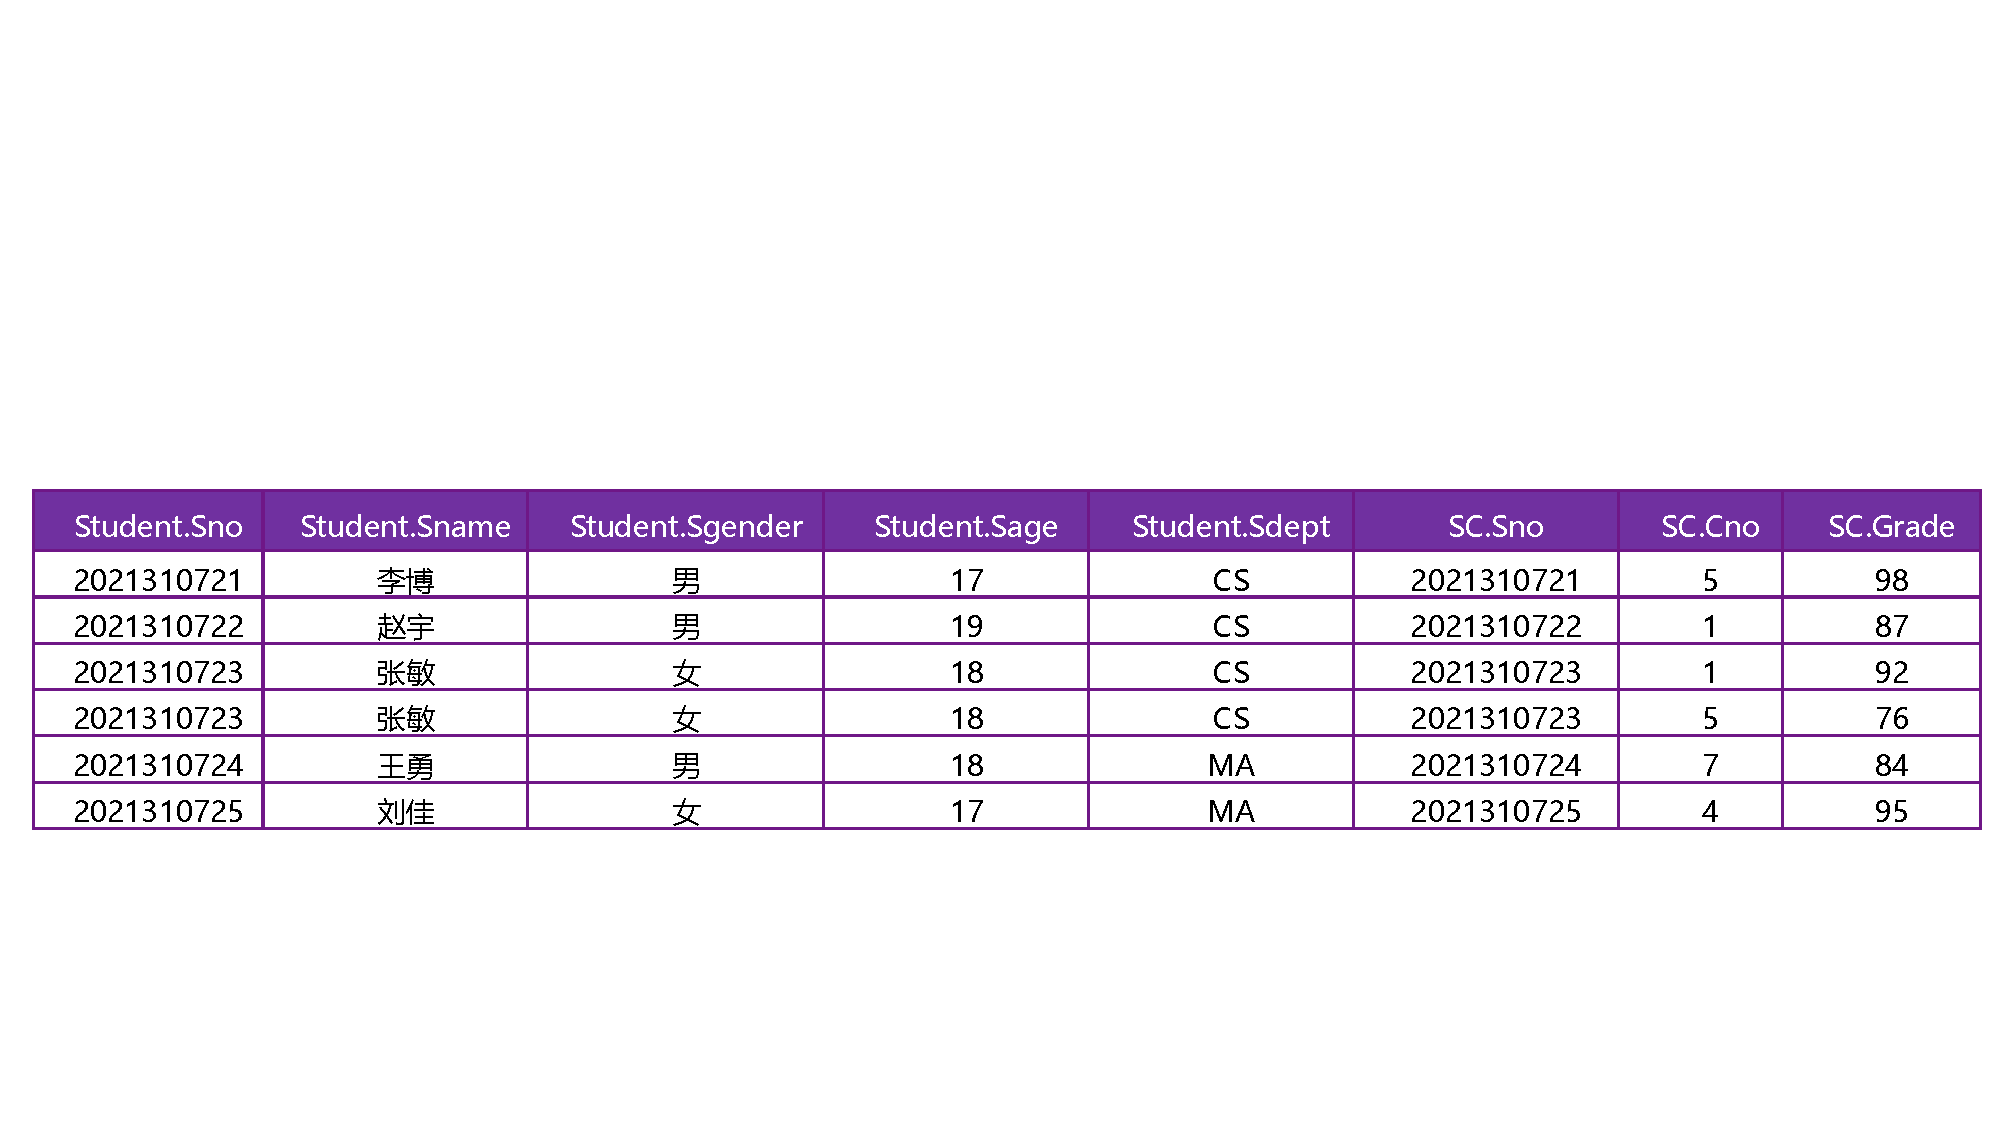
\includegraphics[width=15cm]{images/sec2/2-3_Equijoin.pdf}
        \caption{等值连接}
        \label{fig2-3_1}
    \end{figure}

    而
    $$\mathbf{Student}\bowtie\mathbf{SC}$$
    结果如下:
    \begin{figure}[!htpb]
        \centering
        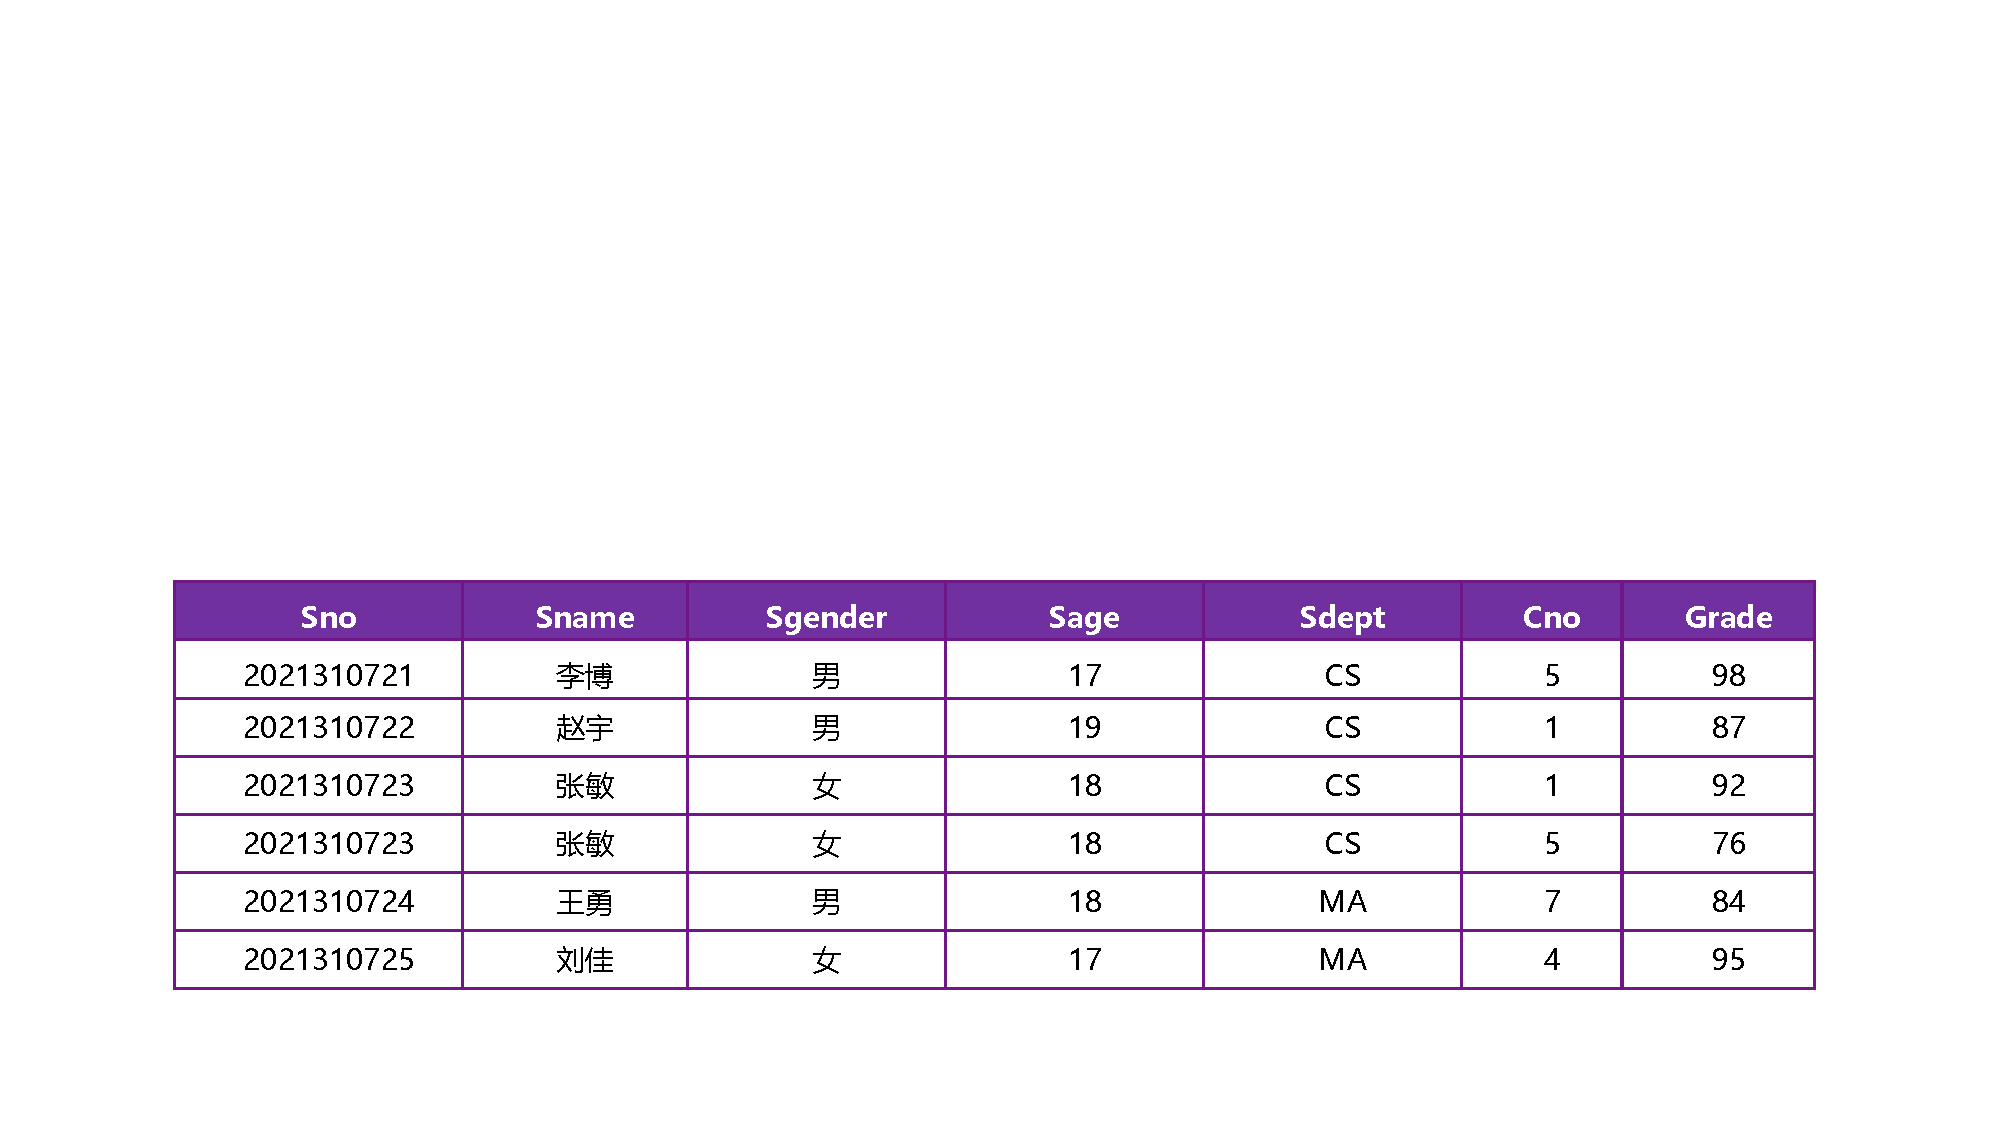
\includegraphics[width=15cm]{images/sec2/2-3_Natural_Join.pdf}
        \caption{自然连接}
        \label{fig2-3_2}
    \end{figure}
\end{note}

\begin{problem}
    关系代数的基本运算有哪些? 如何用这些基本运算来表示其他运算?
\end{problem}

\begin{solution}
    \begin{itemize}
        \item 基本运算:
        \begin{itemize}
            \item 选择($\sigma$):
                  $$\sigma_p(R) = \{t | t \in R \land p(t) = True\}$$
            \item 投影($\Pi$):
                  $$\Pi_{A_1,A_2,\ldots,A_k}(R) = \{t[A_1,A_2,\ldots,A_k] | t \in R\}$$
            \item 并($\bigcup$):
                  $$R\bigcup S = \{t | t\in R \lor t \in S\}$$
            \item 差($-$):
                  $$R - S = \{t | t\in R \land t \notin S\}$$
            \item 笛卡尔积($\times$):
                  $$R \times S = \{(t, q) | t\in R \land q \in S\}$$
        \end{itemize}
        \item 附加运算:
        \begin{itemize}
            \item 交($\bigcap$):
                  $$R\bigcap S = \{t | t\in R \land t \in S\}$$
                  满足:
                  $$R\bigcap S = R - (R - S)$$
            \item 连接($\bowtie$):
                  $$R\bowtie_p S = \{(t, q) | t \in R \land q \in S \land p\left((t, q)\right) = True\}$$
                  满足:
                  $$R\bowtie_p S = \sigma_p(R \times S)$$
            \item 除($\div$): \\
                  设$R(A_1,A_2,\ldots,A_m, B_1,B_2,\ldots,B_n)$和$S(B_1,B_2,\ldots,B_n, C_1,C_2,\ldots,C_k)$ 是两个关系,则$R \div S$的属性为$A_1,A_2,\ldots,A_m$,且:
                  $$R \div S = \{t | t\in \Pi_{A_1,A_2,\ldots,A_m}(R) \land (\forall q \in \Pi_{B_1,B_2,\ldots,B_n}(S), (t, q) \in R)\}$$
                  满足:
                  $$R \div S = \Pi_{A_1,A_2,\ldots,A_m}(R) - \Pi_{A_1,A_2,\ldots,A_m}((\Pi_{A_1,A_2,\ldots,A_m}(R) \times \Pi_{B_1,B_2,\ldots,B_n}(S)) - R)$$
        \end{itemize}
    \end{itemize}
\end{solution}

% \newpage
% \section{第x章作业}
% % 计数器置零
% \setcounter{problemname}{0}

% \begin{problem}

% \end{problem}

% \begin{solution}

% \end{solution}

\end{document}